%====================================================================================
\section[MCG]{Mínimos cuadrados generalizados}
%====================================================================================

\begin{frame}{Tratamiento}
	Después de la prueba, si detectamos la presencia de heterocedasticidad, tenemos los siguientes pasos para el tratamiento.
		\begin{enumerate}
			\item Si nos interesa solo la inferencia, basta con calcular la varianza del estimador excluyendo el supuesto de homocedasticidad \textsf{[Sugerencia de STATA: ayuda a la regresión]}. Un estimador consistente es el estimador de varianza robusta de White. (sugerimos tener una muestra grande para este tratamiento).
			\item Si estamos interesados en la predicción en una muestra pequeña, debe utilizar el estimador de mínimos cuadrados generalizados (MCG o GLS).
		\end{enumerate}
\end{frame}
%---------------------------------------------------
\begin{frame}{Tratamiento \#1: Varianza Robusta de White}
	Recuerde que la varianza del estimador es (en el caso de solo 1 regresor)
		\begin{align*}
			E[\widehat{\beta}_1 - \beta_1]^2 & = E\left[ \frac{\sum_{i=1}^{n}(x - \overline{x})u}{\sum_{i=1}^{n}(x - \overline{x})^2} \right]^2\\
			& = \frac{\sum_{i=1}^{n}(x - \overline{x})^2 E(u^2|x)}{\left[\sum_{i=1}^{n}(x - \overline{x})^2\right]^2}
		\end{align*}
	Como sabe, $E(u^2)$ ya no es una constante entre las observaciones (heterocedasticidad). White H. (1980) sugiere construir la varianza del estimador asumiendo $E (u^2|x)=u^2$
\end{frame}
%---------------------------------------------------
\begin{frame}{Varianza Robusta de White}
	Entonces, tenemos
		\begin{align*}
			E[\widehat{\beta}_1 - \beta_1]^2 &= \frac{\sum_{i=1}^{n}(x - \overline{x})^2 E(u^2|x)}{\left[\sum_{i=1}^{n}(x - \overline{x})^2\right]^2}\\
			& = \frac{\sum_{i=1}^{n}(x - \overline{x})^2 \widehat{u}^2}{\left[\sum_{i=1}^{n}(x - \overline{x})^2\right]^2}
		\end{align*}
	Finalmente, la expresión anterior es la varianza rebusta de White.
\end{frame}
%---------------------------------------------------
\begin{frame}
	Necesitamos algunas correciones para los grados de libertad (pequeño ajuste de muestra)
		$$Var(\widehat{\beta}_1)^{R} = \frac{1}{n(n-k)} \frac{\sum_{i=1}^{n}(x - \overline{x})^2 \widehat{u}^2}{\left[\frac{\sum_{i=1}^{n}(x-\overline{x})^2}{n}\right]^2}$$
	STATA calcula la varianza robusta como en la expresión anterior.
\end{frame}
%---------------------------------------------------
\begin{frame}{Varianza Robusta de White, Ejemplo 1}
	Tengamos en cuenta el conjunto de datos en el ejemplo \#1. Para considerar la varianza robusta de White, deberíamos escribir -después de declarar la regresión- lo siguiente ``		\colorbox{codegray}{\texttt{, robust}}''.
		\begin{figure}
			\centering
			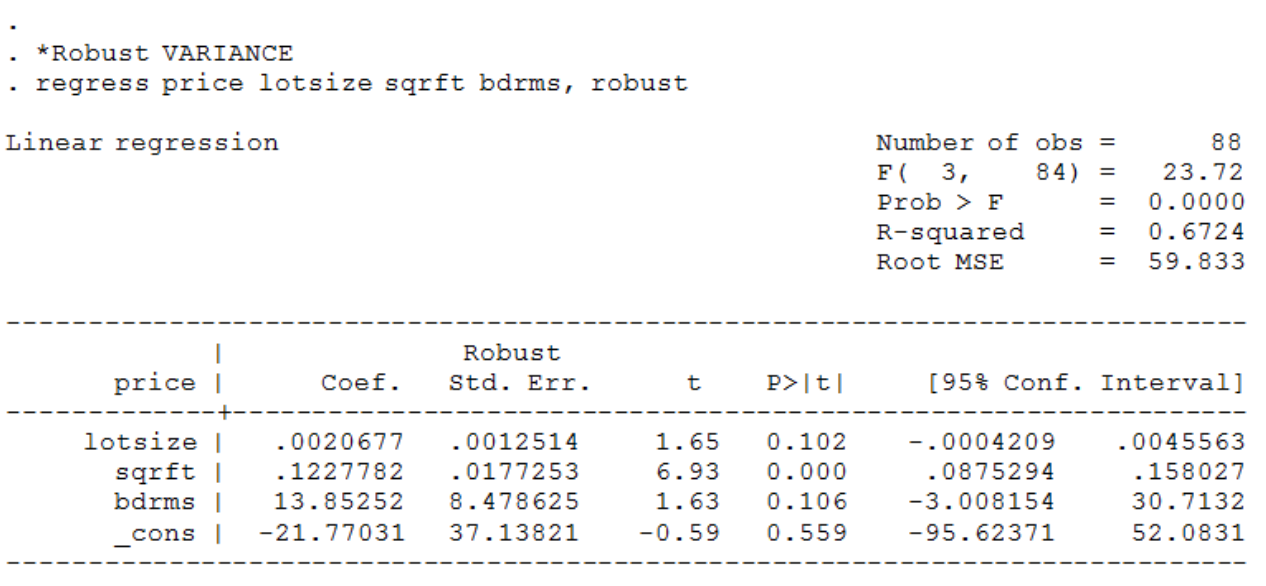
\includegraphics[scale=.30]{fig/white1.png}
		\end{figure}
\end{frame}
%---------------------------------------------------
\begin{frame}{Varianza Robusta de White, Ejemplo 2}
	Tengamos en cuenta el conjunto de datos del ejemplo \#2.
		\begin{figure}
			\centering
			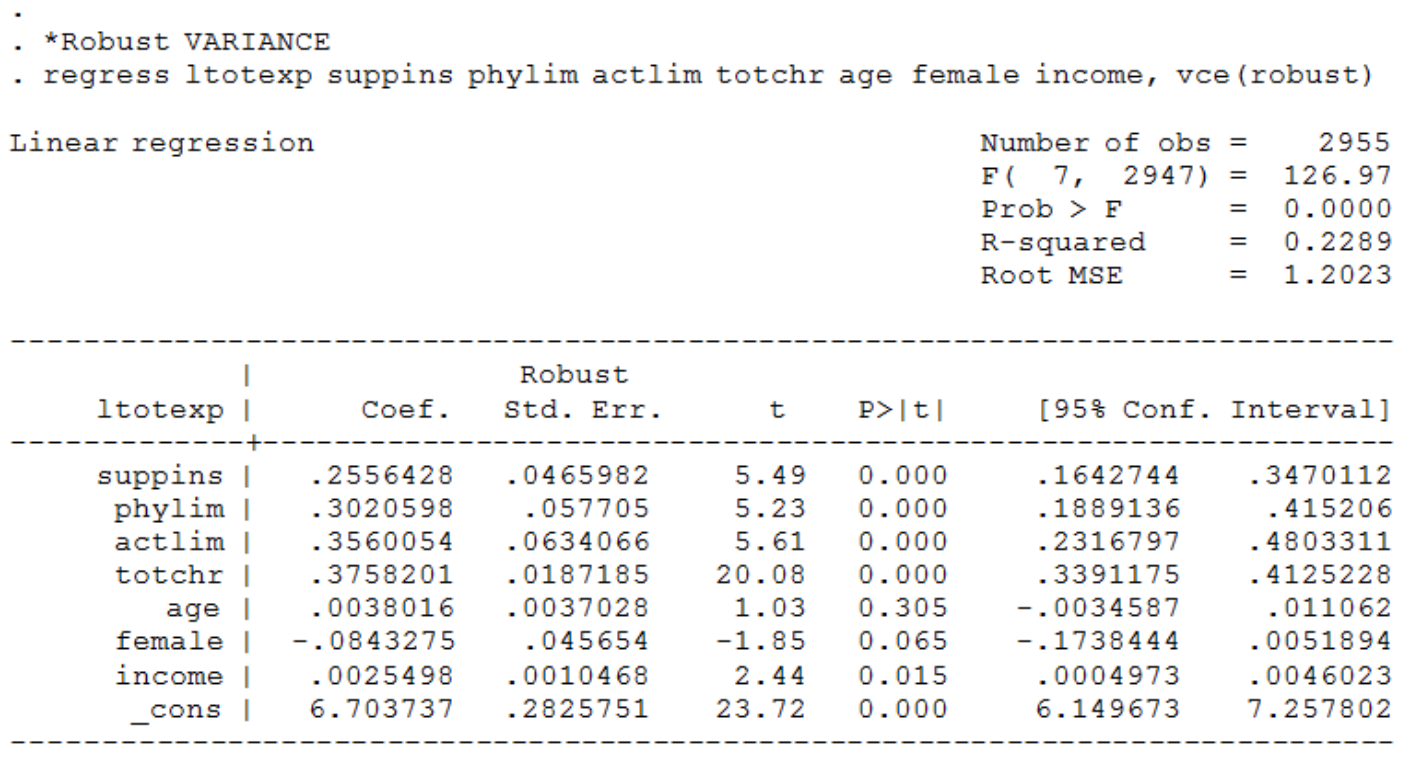
\includegraphics[scale=.30]{fig/white2.png}
		\end{figure}
\end{frame}
%---------------------------------------------------
\begin{frame}{Varianza Robusta de White, Ejemplo 3}
	Tengamos en cuenta el conjunto de datos del ejemplo \#3.
		\begin{figure}
			\centering
			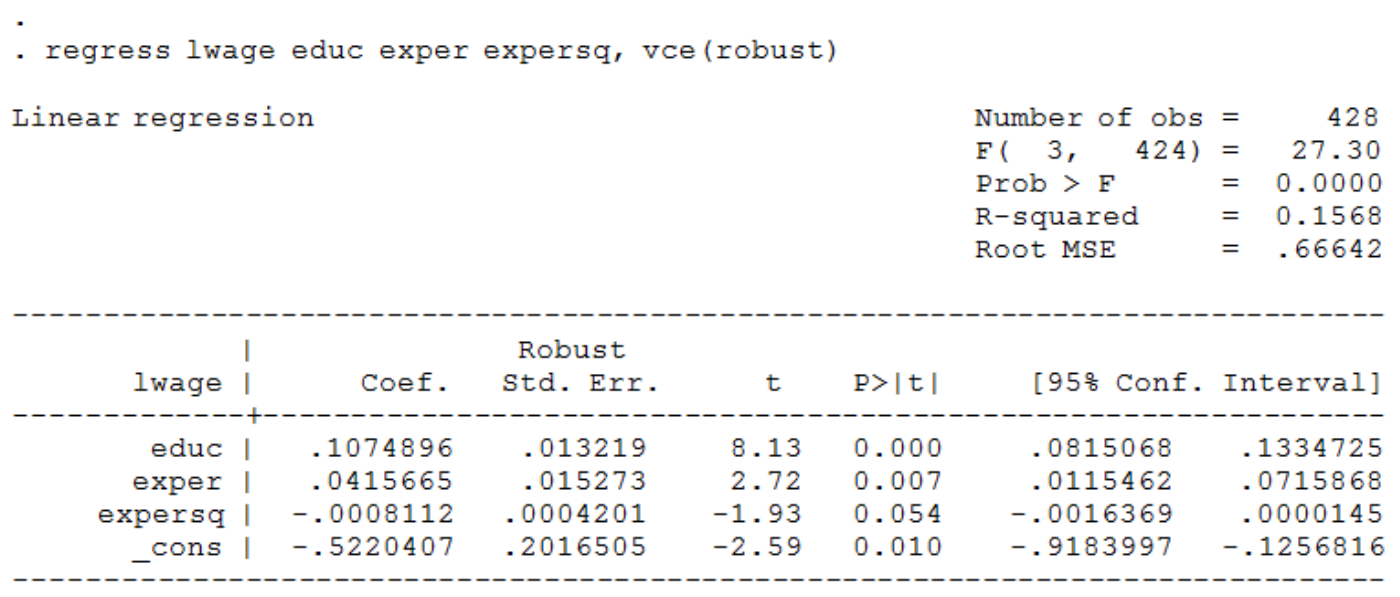
\includegraphics[scale=.30]{fig/white3.png}
		\end{figure}
\end{frame}
%---------------------------------------------------
\begin{frame}{Tratamiento \#2: Mínimos cuadrados ponderados}
	\begin{itemize}
		\item Siempre es posible estimar errores estándar robustos para MCO.
		\item Pero si se conoce la forma funcional de la heterocedasticidad, se pueden obtener estimadores más eficientes que MCO.
		\item La idea básica es transformar el modelo para conseguir errores homocedásticos. Este procedimiento se conoce como Mínimos Cuadrados Ponderados (MCP).
	\end{itemize}
\end{frame}
%---------------------------------------------------
\begin{frame}{Caso: Varianza proporcional a un valor constante}
	\begin{itemize}
		\item En este caso la heterocedastidas puede ser modelado como:
				$$Var(\mu | x)=\sigma^2h(x)$$
		\item Donde se puede representar $h(x)=h_i$.
		\item $E(\mu_i | \sqrt{h_i(x)})=0$, debido $h_i$ es una función de $x$, y $Var(\mu_i | \sqrt{h_i|x})=\sigma^2$, debido que se sabe $Var(\mu | (x))=\sigma^2 h_i$.
		\item Así, si se divide la ecuación de regresión por $\sqrt{h_i}$ se tendrá un modelo donde los errores son homocedásticos.
	\end{itemize}
\end{frame}
%---------------------------------------------------
\begin{frame}{Mínimos Cuadrados Generalizados}
	\begin{itemize}
		\item Estimar la ecuación transformada por MCO es un ejemplo de Mínimos Cuadrados Generalizados (MCG).	
		\item MCG es MELI en este caso.
		\item MCG es un procedimiento de Mínimos Cuadrados Ponderado (MCP) donde cada residuo es ponderado por el recíproco de $Var(\mu|x)$
	\end{itemize}
\end{frame}
%---------------------------------------------------
\begin{frame}{Mínimos Cuadrados Ponderados}
	\begin{itemize}
		\item Mientras que es intuitivo ver la razón por la que se realiza la transformación en MCO para conseguir homocedasticidad, dicha transformación podría ser problemática.	
		\item MCP es un camino para alcanzar el mismo objetivo sin necesidad de hacer la transformación.
		\item La idea es minimizar la suma ponderada de errores al cuadrado (ponderada por $1/h_i$):
				$$\sum_{i=1}^n(y_i-\beta_0-\beta_1 x_{i1}-...-\beta_k x_{ik})^2/h_i$$
				$$\sum_{i=1}^n(y_i^*-\beta_0 x_{i0}^*-\beta_1 x_{i1}^*-...-\beta_k x_{ik}^*)^2$$
	\end{itemize}
\end{frame}
%---------------------------------------------------
\begin{frame}{Mínimos Cuadrados Ponderados}
	\begin{itemize}
		\item MCP es el camino adecuado si se conoce como es $Var(\mu|x)$.	
		\item Aunque en la mayoría de los casos no conocemos la forma funcional de la heterocedasticidad.
		\item Un ejemplo donde si es conocido el patrón de heterocedasticidad es cuando los datos están agregados.
		\item En ese caso se puede ponderar cada observación agregada por el recíproco de la cantidad de individuos en cada grupo.
	\end{itemize}
\end{frame}
%---------------------------------------------------
\begin{frame}{MCG factibles}
	\begin{itemize}
		\item Lo usual es el caso donde no sepamos la forma funcional de la heterocedasticidad.
		\item En este caso, necesitamos estimar $h(x_i)$-
		\item Tipicamente se asume un forma funcional flexible:
				$$Var(\mu | x)=\sigma^2 exp(\alpha_0+\alpha_1 x_1+...+\alpha_k x_k)$$
		\item El objetivo entonces es estimar los $\alpha$.
	\end{itemize}
\end{frame}
%---------------------------------------------------
\begin{frame}{MCG factibles}
	\begin{itemize}
		\item El supuesto implica que:
				$$\mu^2=\sigma^2 exp(\alpha_0+\alpha_1 x_1+...+\alpha_k x_k)v$$
		\item Donde $E(v|x)=1$, que implica $E(v)=1$	
		\item $ln(\mu^2)=\alpha_0+\alpha_1 x_1+...+\alpha_k x_k+\epsilon$
		\item Donde $E(\epsilon)=1$ y $\epsilon$ es independiente de $x$.
		\item Ahora, sabiendo que $\hat \mu$ es un estimado de $\mu$, podemos estimar esto por MCO.
	\end{itemize}
\end{frame}
%---------------------------------------------------
\begin{frame}{MCG factibles}
	\begin{itemize}
		\item Así, un estimado de $h$ es obtenido como $\hat h=exp(\hat g)$, y el recíproco de esto es nuestro ponderador.
		\item Resumiendo:
		\item Estimar el modelo original MCO, guardar los residuos $\hat\mu$, elevarlos al cuadrado, y tomar el logaritmo.
		.
		\item Regresionar $ln(\hat \mu^2)$ sobre todas las variables independientes y obtener los valores estimados $\hat g$.
		\item Estimar MCG usando $1/exp(\hat g)$ como ponderador. 
	\end{itemize}
\end{frame}
%---------------------------------------------------
\begin{frame}{Consideraciones}
	\begin{enumerate}
		\item MCO sigue siendo insesgado y coherente.
		\item Después de comprobar que existe evidencia de heterocedasticidad en nuestro modelo, necesitamos tratamiento.
		
		\item Hay 2 tratamientos para el problema (reducción) de heterocedasticidad: GLS o calcular la opción robusta de White usando STATA. Nota: Heterocedasticidad no deseparece, se asume.
		
		\item GLS debe ser factible; necesitamos conocer el verdadero patrón de heterocedasticidad.
		
		\item El uso de una opción robusta en STATA es factible; podemos calcular la varianza de los estimadores de MCO asumiendo heterocedasticidad.
		
		\item Los errores estándar deben corregirse asumiendo heterocedasticidad, entonces estamos listos para hacer inferencias.
	\end{enumerate}
\end{frame}